\documentclass[tikz,border=5pt]{standalone}
\usepackage{amsmath}
\usetikzlibrary{arrows.meta,positioning,fit,calc}

\begin{document}
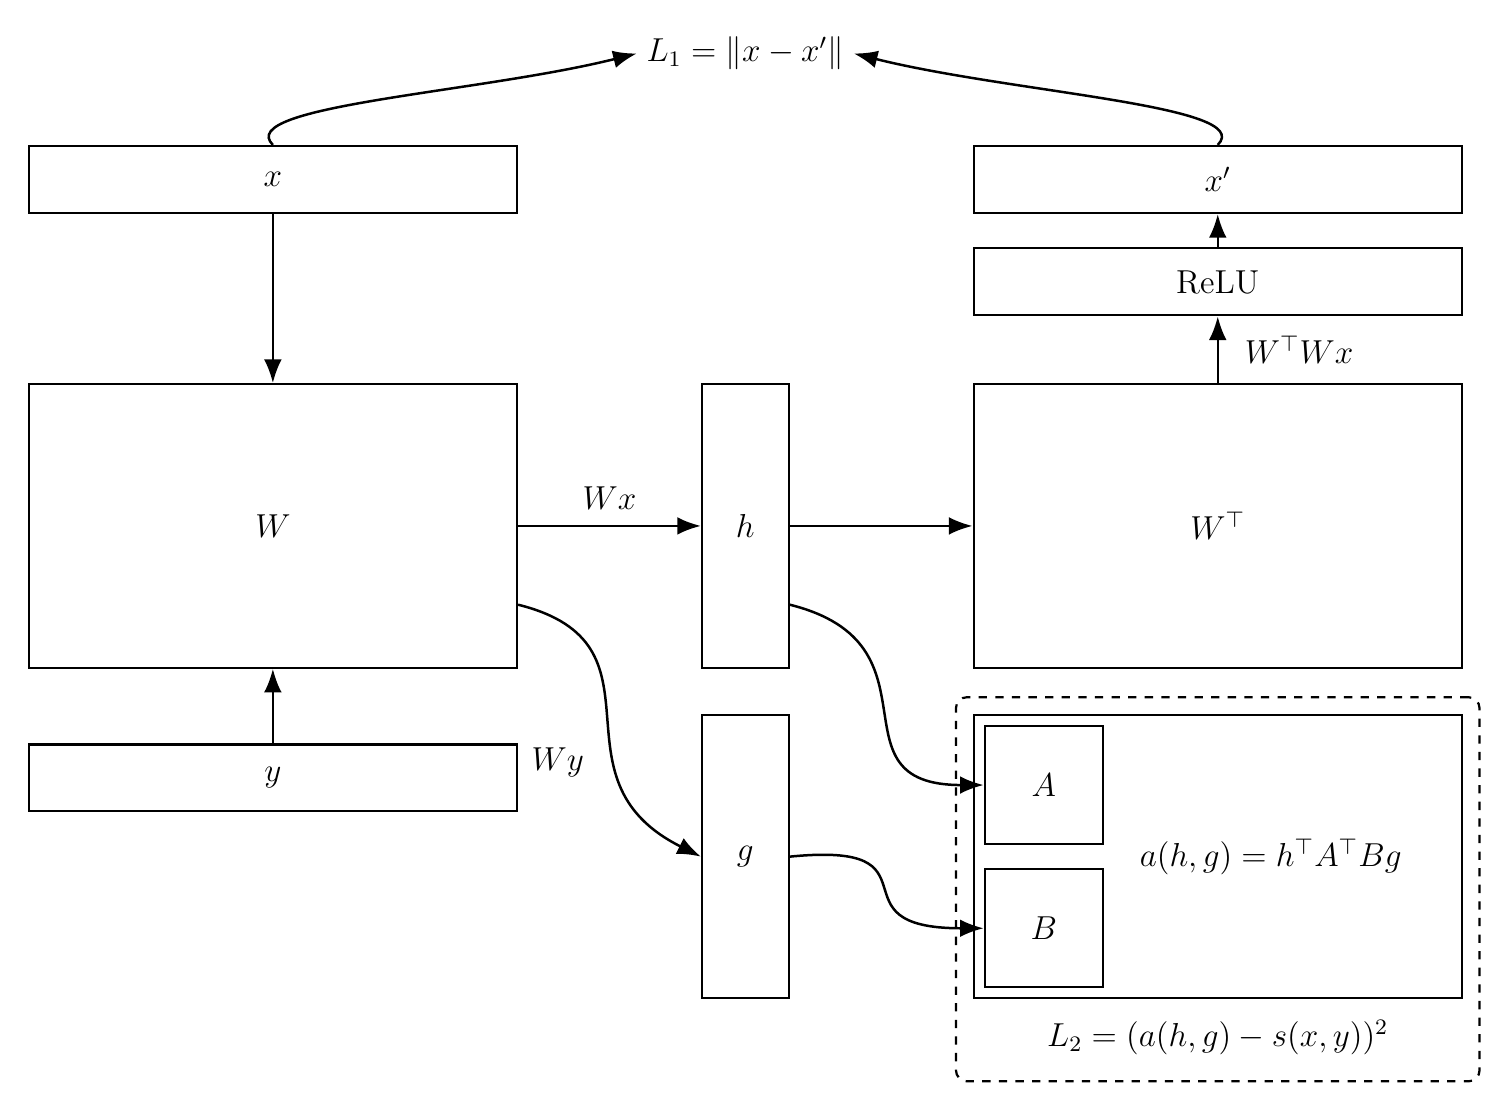
\begin{tikzpicture}[font=\large]
  %----- styles
  \tikzset{
    box/.style   ={draw,thick,minimum width=6.2cm,minimum height=3.6cm,align=center},
    slim/.style  ={draw,thick,minimum width=1.1cm,minimum height=3.6cm,align=center},
    var/.style   ={draw,thick,minimum width=6.2cm,minimum height=0.85cm}, % rectangular, same width as W
    slab/.style  ={draw,thick,minimum width=6.2cm,minimum height=0.85cm}, % same width as W
    arrow/.style ={-{Latex[length=3mm]},line width=0.9pt},
    dashedbox/.style ={draw,dashed,rounded corners,inner sep=6pt,thick},
    smallsq/.style={draw,thick,minimum width=1.5cm,minimum height=1.5cm}
  }

  %----- nodes
  % top row: x and x'
  \node[var] (x)  at (-6, 3.8) {$x$};
  \node[var] (xp) at ( 6, 3.8) {$x'$};

  % main blocks: W, h, W^T, ReLU
  \node[box]  (W)   at (-6,-0.6) {$W$};
  \node[slim] (h)   at ( 0,-0.6) {$h$};
  \node[box]  (Wt)  at ( 6,-0.6) {$W^{\top}$};
  \node[slab] (relu)at ( 6, 2.5) {ReLU};

  % new nodes: y below W (same size as x), g below h (same size as h)
  \node[var]  (y) at (-6,-3.8) {$y$};
  \node[slim] (g) at ( 0,-4.8) {$g$};

  % new node: big box below W^T, aligned with g
  \node[box,align=left] (ybox) at (6,-4.8) {};

  % text label shifted to the right side of ybox
  \node[anchor=west] at ($(ybox.west)+(2.0,0)$) {$a(h,g) = h^\top A^\top B g$};

  % small square boxes inside ybox (left side, vertically aligned)
  \node[smallsq,anchor=north west] (sq1) at ([xshift=4pt,yshift=-4pt]ybox.north west) {$A$};
  \node[smallsq,anchor=south west] (sq2) at ([xshift=4pt,yshift=4pt]ybox.south west) {$B$};

  % label directly below the new box
  \node (L2) [below=4pt of ybox] {$L_2 = (a(h,g) - s(x,y))^2$};

  % dashed group box around ybox + L2
  \node[dashedbox,fit=(ybox)(L2)] {};

  %----- connections (existing)
  \draw[arrow] (x.south) -- (W.north);
  \draw[arrow] (W.east) -- node[above=2pt] {$Wx$} (h.west);
  \draw[arrow] (h.east) -- (Wt.west);
  \draw[arrow] (Wt.north) -- (relu.south) node[midway,right=6pt] {$W^{\top} W x$};
  \draw[arrow] (relu.north) -- (xp.south);

  %----- new connections
  % y -> W (arrow upward into W)
  \draw[arrow] (y.north) -- (W.south);

  % W -> g (arrow leaves W lower, label Wy)
  \coordinate (Wexit) at ($(W.east)+(0,-1.0)$);
  \draw[arrow] (Wexit) .. controls +(2,-0.5) and +(-2,1.0) .. (g.west);
  \node[anchor=east] at ($(Wexit)!0.5!(g.west)+(-0.2,-0.4)$) {$Wy$};

  % h -> A (curved arrow into midpoint of sq1)
  \coordinate (hexit) at ($(h.east)+(0,-1.0)$);
  \draw[arrow] (hexit) .. controls +(2,-0.5) and +(-2,0.0) .. (sq1.west);

  % g -> B (curved arrow into midpoint of sq2)
  \coordinate (gexit) at ($(g.east)+(0,0)$);
  \draw[arrow] (gexit) .. controls +(2,0.2) and +(-2,0.0) .. (sq2.west);

  %----- loss label and concave-downward arrows
  \node (loss) at (0,5.4) {$L_1=\lVert x - x' \rVert$};
  \draw[arrow] (x.north)  .. controls +(-0.5,0.5) and +(-2,-0.5) .. (loss.west);
  \draw[arrow] (xp.north) .. controls +( 0.5,0.5) and +( 2,-0.5) .. (loss.east);
\end{tikzpicture}
\end{document}
